\documentclass[a4paper]{article}
\usepackage{polski}
\usepackage[utf8]{inputenc}
\usepackage{url}
\usepackage{navigator}
\usepackage{graphicx}
\usepackage{float}
\embeddedfile{main}{./main.tex}
\usepackage{listings}
\lstdefinestyle{java}
{basicstyle=\ttfamily\supertiny,language=java,tabsize=4,showspaces=false,showstringspaces=false,xleftmargin=0cm,basicstyle=\ttfamily,columns=fullflexible,keepspaces=true,frame=none,breaklines=true}
\lstdefinestyle{xml}
{basicstyle=\ttfamily\supertiny,language=xml,tabsize=4,showspaces=false,showstringspaces=false,xleftmargin=0cm,basicstyle=\ttfamily,columns=fullflexible,keepspaces=true,frame=none,breaklines=true}

\title{\bf{Aplikacja mobilna dla biegacza - GitFitScrub}}
\author{{\em Michał Ptak, Katarzyna Poręba, Jan Michalik}}
\date{}

\begin{document}

\begin{titlepage}
\maketitle
\thispagestyle{empty}
\bigskip
\begin{center}
Zespołowe przedsięwzięcie inżynierskie\\[2mm]

Informatyka\\[2mm]

Rok. akad. 2017/2018, sem. I\\[2mm]

Prowadzący: dr hab. Marcin Mazur
\end{center}
\end{titlepage}

\tableofcontents
\thispagestyle{empty}

\newpage

\section{Opis projektu}

\subsection{Członkowie zespołu}

\begin{enumerate}
\item Michał Ptak (kierownik projektu).
\item Katarzyna Poręba.
\item Jan Michalik.
\end{enumerate}

\subsection{Cel projektu (produkt)}

Naszym celem jest zbudowanie aplikacji mobilnej na system operacyjny Android przy użyciu map Google, która pobiera informacje poruszającej się osoby z modułu GPS i gromadzi statystyki dotyczące długości trasy, prędkości czy spalanych kalorii, a także zapisuje poczynania w bazie danych.

\subsection{Potencjalny odbiorca produktu (klient)}

% Określić potencjalnego klienta (wraz z uzasadnieniem).
Klient jest biegaczem oczekującym w pełni darmowej aplikacji bez reklam, która będzie śledzić trasę, po której się porusza oraz wyświetlać aktualne statystyki. Aktualnie żadna dostępna na rynku aplikacja nie spełnia odbiorcy produktu.

\subsection{Metodyka}

Projekt będzie realizowany przy użyciu (zaadaptowanej do istniejących warunków) metodyki {\em Scrum}.

\section{Wymagania użytkownika}
%<<Przedstawić listę wymagań użytkownika w postaci ,,historyjek'' (User stories). Każda historyjka powinna opisywać jedną cechę systemu. Struktura: As a [type of user], I want [to perform some task] so that I can [achieve some goal/benefit/value] (zob. np. \cite{us}).>>

\subsection{User story 1}
Jako użytkownik, chcę mieć dostęp do mapy podczas treningu, aby widzieć jaką trasą się poruszam.

\subsection{User story 2}
Jako użytkownik, chcę mieć możliwość wciśnięcia przycisku "Start", aby rozpocząć pomiar.

\subsection{User story 3}
Jako użytkownik, chcę mieć możliwość wciśnięcia przycisku "Stop", aby zakończyć pomiar.

\subsection{User story 4}
Jako użytkownik, chcę widzieć czas, który upłynął od rozpoczęcia pomiaru biegu, aby kontrolować jego upływ.

\subsection{User story 5}
Jako użytkownik, chcę widzieć przebyty dystans, aby kontrolować jego długość.

\subsection{User story 6}
Jako użytkownik, chcę widzieć prędkość chwilową, z jaką się poruszam, aby zachować określone tempo.

\subsection{User story 7}
Jako użytkownik, chcę zobaczyć podsumowanie odbytego treningu, aby ocenić jego rezultat.
%ocena treningu

\subsection{User story 8}
Jako użytkownik, chcę mieć możliwość włączenia trybu nocnego, aby zmniejszyć zmęczenie wzroku po zmroku.

\subsection{User story 9 (opcjonalne)}
Jako użytkownik niezarejestrowany, chcę mieć możliwość rejestracji, aby móc się zalogować.

\subsection{User story 10 (opcjonalne)}
Jako użytkownik zarejestrowany, chcę mieć możliwość zalogowania się, aby móc korzystać ze wszystkich funkcji aplikacji.

\subsection{User story 11 (opcjonalne)}
Jako użytkownik zalogowany, chcę mieć możliwość wylogowania się, aby móc zalogować się na inne konto.

\subsection{User story 12 (opcjonalne)}
Jako użytkownik zalogowany, chcę mieć możliwość ustawienia swojego pseudonimu, aby wiedzieć czy jestem zalogowany na swoim koncie.

\subsection{User story 13 (opcjonalne)}
Jako użytkownik zalogowany, chcę aby statystyki z odbytych treningów zostały zapisane w historii, celem ich późniejszej analizy.

\subsection{User story 14 (opcjonalne)}
Jako użytkownik zalogowany, chcę widzieć w statystykach spalone kalorie, by móc dostosować swoją dietę.

\subsection{User story 15 (opcjonalne)}
Jako użytkownik zalogowany, chcę mieć możliwość usunięcia (całej lub części) historii treningów, aby rozpocząć nowy cykl treningowy.

\subsection{User story 16 (opcjonalne)}
Jako użytkownik zalogowany, chcę by aplikacja pamiętała ostatnio użyty login, aby nie wpisywać go ręcznie przy kolejnym logowaniu.

\subsection{User story 17 (opcjonalne)}
Jako użytkownik zalogowany, chcę mieć możliwość ręcznego zatrzymania pomiaru czasu oraz dystansu, aby napotkane przeszkody (np. czerwone światło) nie fałszowały statystyk.

\subsection{User story 18 (opcjonalne)}
Jako użytkownik zalogowany, chcę mieć możliwość podjęcia wyzwania pokonania określonych odległości (np. z Ziemi do Księżyca), aby mieć motywację do kontynuowania treningu.

\subsection{User story 19 (opcjonalne)}
Jako użytkownik zalogowany, chce mieć możliwość udostępnienia swoich osiągnięć na portalach społecznościowych, aby podzielić się rezultatami ze znajomymi.

\subsection{User story 20 (opcjonalne)}
Jako użytkownik, chcę mieć możliwość ustawienia powiadomień po określonym przez siebie odcinku trasy, by nie być zmuszonym do ciągłego sprawdzania aplikacji.

\section{Harmonogram}

\subsection{Rejestr zadań (Product Backlog)}

\begin{itemize}
	\item Data rozpoczęcia: 24.10.2017.
	\item Data zakończenia: 31.10.2017.
\end{itemize}

\subsection{Sprint 1}

\begin{itemize}
\item Data rozpoczęcia: 31.10.2017.
\item Data zakończenia: 14.11.2017.
\item Scrum Master: Katarzyna Poręba.
\item Product Owner: Michał Ptak.
\item Development Team: Michał Ptak, Katarzyna Poręba, Jan Michalik.
\end{itemize}

\subsection{Sprint 2}

\begin{itemize}
\item Data rozpoczęcia: 14.11.2017.
\item Data zakończenia: 28.11.2017.
\item Scrum Master: Michał Ptak.
\item Product Owner: Jan Michalik.
\item Development Team: Michał Ptak, Katarzyna Poręba, Jan Michalik.
\end{itemize}

\subsection{Sprint 3}

\begin{itemize}
\item Data rozpoczęcia: 28.11.2017.
\item Data zakończenia: 12.12.2017.
\item Scrum Master: Jan Michalik.
\item Product Owner: Katarzyna Poręba.
\item Development Team: Michał Ptak, Katarzyna Poręba, Jan Michalik.
\end{itemize}

\subsection{Sprint 4}

\begin{itemize}
\item Data rozpoczęcia: 12.12.2017.
\item Data zakończenia: 19.12.2017.
\item Scrum Master: Katarzyna Poręba.
\item Product Owner: Michał Ptak.
\item Development Team: Michał Ptak, Katarzyna Poręba, Jan Michalik.
\end{itemize}

\subsection{Sprint 5}

\begin{itemize}
\item Data rozpoczęcia: 19.12.2017.
\item Data zakończenia: 09.01.2018.
\item Scrum Master: Michał Ptak.
\item Product Owner: Jan Michalik.
\item Development Team: Michał Ptak, Katarzyna Poręba, Jan Michalik.
\end{itemize}

\subsection{Sprint 6}

\begin{itemize}
\item Data rozpoczęcia: 09.01.2018.
\item Data zakończenia: 16.01.2018.
\item Scrum Master: Michał Ptak.
\item Product Owner: Katarzyna Poręba.
\item Development Team: Michał Ptak, Katarzyna Poręba, Jan Michalik.
\end{itemize}

\section{Product Backlog}

\subsection{Backlog Item 1}
\paragraph{Tytuł zadania.} Przygotowanie zestawu narzędzi SDK.
\paragraph{Opis zadania.} Dodanie do zestawu SDK: Google Services, nową dystrybucję Androida (wersja Oreo), debugowanie poprzez USB. Wykonanie prostego programu testującego działanie kompilatora oraz zainstalowanej dystrybucji.
\paragraph{Priorytet.} 10.
\paragraph{Definition of Done.} Poprawne zainstalowanie wybranych narzędzi SDK na stacjach roboczych.

\subsection{Backlog Item 2}
\paragraph{Tytuł zadania.} Stworzenie wstępnej wersji aplikacji.
\paragraph{Opis zadania.} Utworzenie aplikacji zawierającej puste menu główne.
\paragraph{Priorytet.} 10.
\paragraph{Definition of Done.} Aplikacja po uruchomieniu wyświetla menu główne.

\subsection{Backlog Item 3}
\paragraph{Tytuł zadania.} Dodanie uprawnień aplikacji.
\paragraph{Opis zadania.} Dodanie uprawnień aplikacji do korzystania z Internetu i modułu GPS, co weryfikowane jest w \ref{bl4}.
\paragraph{Priorytet.} 10.
\paragraph{Definition of Done.} Aplikacja posiada możliwość korzystania z Internetu i nawigacji.

\subsection{Backlog Item 4}
\label{bl4}
\paragraph{Tytuł zadania.} Stworzenie przycisku "Rozpocznij" w menu głównym oraz nadanie mu funkcjonalności.
\paragraph{Opis zadania.} Utworzenie nowej aktywności uruchamiającej mapę Google i nanoszącej na nią znacznika wskazującego geolokalizację użytkownika. Utworzenie przycisku i nadanie mu akcji uruchomienia tejże aktywności. Zaprojektowanie szaty graficznej menu głównego i stworzenie logo oraz ikony aplikacji.
\paragraph{Priorytet.} 8.
\paragraph{Definition of Done.} Po naciśnięciu przycisku "Rozpocznij" uruchomi moduł GPS i pokaże znacznik wskazujący aktualną pozycję użytkownika na mapie.

\subsection{Backlog Item 5}
\paragraph{Tytuł zadania.} Stworzenie alertu o braku aktywacji modułu GPS.
\paragraph{Opis zadania.} Utworzenie metody w klasie MapsActivity sprawdzającej stan aktywności modułu GPS, oraz powiadamiającej użytkownika o wyłączonym GPS-ie. Po zatwierdzeniu alertu aplikacja przenosi użytkownika do ustawień systemowych Android™.
\paragraph{Priorytet.} 6.
\paragraph{Definition of Done.}

\subsection{Backlog Item 6}
\paragraph{Tytuł zadania.} Pobranie informacji z modułu GPS.
\paragraph{Opis zadania.} Utworzenie nowej aktywności pobierającej surowe dane geograficzne oraz gromadzenie ich w pamięci operacyjnej. Weryfikacja poprawności uzyskanych danych poprzez wydruk w konsoli dewelopera.
\paragraph{Priorytet.} 9.
\paragraph{Definition of Done.} Surowe dane geograficzne znajdują się w pamięci operacyjnej systemu.

\subsection{Backlog Item 7}
\paragraph{Tytuł zadania.} Stworzenie przycisku "Rozpocznij nowy trening" oraz nadanie mu funkcjonalności.
\paragraph{Opis zadania.} Utworzenie nowej aktywności wywołującej metodę odpowiadającej za wysunięcie pustego panelu statystyk.
\paragraph{Priorytet.} 9.
\paragraph{Definition of Done.} U dołu mapy, wyświetlającej naszą aktualną pozycję, widnieje przycisk rozpoczynający trening, który po naciśnięciu wysunie panel ze statystykami.

\subsection{Backlog Item 8}
\paragraph{Tytuł zadania.} Przetworzenie zgromadzonych informacji.
\paragraph{Opis zadania.} Utworzenie funkcji kalkulujących dystans, prędkość, ilość spalonych kcal i upływ czasu, które zostają wywołane po naciśnięciu przycisku "Rozpocznij nowy trening". Przechowywanie wartości zwracanych przez funkcje w pamięci operacyjnej systemu.
\paragraph{Priorytet.} 9.
\paragraph{Definition of Done.} Dane zwracane przez funkcję mają odwzorowanie w rzeczywistości.

\subsection{Backlog Item 9}
\paragraph{Tytuł zadania.} Modyfikacja panelu zawierającego statystyki aktualnego treningu.
\paragraph{Opis zadania.} Utworzenie nowej aktywności pobierającej przetworzone dane geograficzne. Określenie pozycji wyświetlanych parametrów typu: czas, dystans, prędkość. Sprzężenie tejże aktywności z pozycjami statystyk celem ich wyświetlenia użytkownikowi.
\paragraph{Priorytet.} 7.
\paragraph{Definition of Done.} Wyświetlenie przetworzonych informacji pobranych z modułu GPS.

\subsection{Backlog Item 10}
\paragraph{Tytuł zadania.} Rysowanie polilinii na mapie.
\paragraph{Opis zadania.} Utworzenie metody tworzącej ślad na mapie przemieszczającego się użytkownika, na podstawie informacji z modułu GPS.
\paragraph{Priorytet.} 8.
\paragraph{Definition of Done.}

\subsection{Backlog Item 11}
\paragraph{Tytuł zadania.} Stworzenie przycisku "Zakończ trening" oraz nadanie mu funkcjonalności.
\paragraph{Opis zadania.} Utworzenie nowej aktywności wywołującej metodę odpowiadającej za zakończenie pomiarów i rysowanie polilinii na mapie, a także otwierającej panel z podsumowaniem treningu --- wszystkich wyznaczonych statystyk.
\paragraph{Priorytet.} 9.
\paragraph{Definition of Done.} Po naciśnięciu "Zakończ trening" aplikacja zatrzymuje pomiary i wyświetla podsumowanie treningu.

\subsection{Backlog Item 12}
\paragraph{Tytuł zadania.} Stworzenie przycisku "Ustawienia" w menu głównym oraz nadanie mu funkcjonalności.
\paragraph{Opis zadania.} Stworzenie nowej aktywności uruchamiającej listę dostępnych ustawień.
\paragraph{Priorytet.} 5.
\paragraph{Definition of Done.} Po naciśnięciu przycisku "Ustawienia" w menu głównym otwiera się lista ustawień.

\subsection{Backlog Item 13}
\paragraph{Tytuł zadania.} Dodanie funkcji trybu nocnego do panelu ustawień.
\paragraph{Opis zadania.} Dodanie przełącznika do panelu ustawień zmieniającego styl mapy oraz panelu statystyk na "nocny" lub "dzienny".
\paragraph{Priorytet.} 5.
\paragraph{Definition of Done.} Po naciśnięciu przełącznika mapa oraz panel statystyk zmieniają styl wyglądu na "dzienny" lub "nocny".

\subsection{Backlog Item 14 (opcjonalne)}
\paragraph{Tytuł zadania.} Dodanie aktywności logowania użytkownika.
\paragraph{Opis zadania.} Dodanie możliwości logowania za pośrednictwem konta Google.
\paragraph{Priorytet.} 6.
\paragraph{Definition of Done.} Konto Google użytkownika zostaje połączone z aplikacją GitFitScrub. Poprawność połączenia weryfikowana na podstawie strony "Aplikacje połączone z Twoim kontem" \url{https://myaccount.google.com/permissions}.

\subsection{Backlog Item 15 (opcjonalne)}
\paragraph{Tytuł zadania.} Dodanie aktywności wylogowania użytkownika.
\paragraph{Opis zadania.} Dodanie możliwości wylogowania się z konta Google.
\paragraph{Priorytet.} 6.
\paragraph{Definition of Done.} Konto Google użytkownika zostaje rozłączone z aplikacji GitFitScrub.

\subsection{Backlog Item 16 (opcjonalne)}
\paragraph{Tytuł zadania.} Stworzenie przycisku "Zaloguj" w ustawieniach oraz nadanie mu funkcjonalności.
\paragraph{Opis zadania.} Wywołanie metody połączenia się z kontem Google.
\paragraph{Priorytet.} 5.
\paragraph{Definition of Done.} Po wprowadzeniu poprawnych danych użytkownik zostaje pomyślnie uwierzytelniony.

\subsection{Backlog Item 17 (opcjonalne)}
\paragraph{Tytuł zadania.} Stworzenie przycisku "Wyloguj" w ustawieniach oraz nadanie mu funkcjonalności.
\paragraph{Opis zadania.} Wywołanie metody rozłączenia się z kontem Google.
\paragraph{Priorytet.} 5.
\paragraph{Definition of Done.} Po naciśnięciu przycisku użytkownik zostaje pomyślnie wylogowany.

\subsection{Backlog Item 18 (opcjonalne)}
\paragraph{Tytuł zadania.} Utworzenie miejsca, w którym archiwizowane będą statystyki użytkownika zalogowanego.
\paragraph{Opis zadania.} Wygenerowanie certyfikatu do autoryzacji komunikacji aplikacji z chmurą. Sprawdzenie komunikacji baza - aplikacja poprzez wysłanie testowych informacji na chmurę.
\paragraph{Priorytet.} 5.
\paragraph{Definition of Done.} Aplikacja bez przeszkód komunikuje się z bazą danych w chmurze Google Drive.

\subsection{Backlog Item 19 (opcjonalne)}
\paragraph{Tytuł zadania.} Ustawienie pseudonimu użytkownika zalogowanego.
\paragraph{Opis zadania.} Utworzenie nowego pola w ustawieniach, którego celem będzie ustawienie aktualnego pseudonimu.
\paragraph{Priorytet.} 3.
\paragraph{Definition of Done.} Użytkownik zalogowany ma możliwość ustawienia pseudonimu.

\subsection{Backlog Item 20 (opcjonalne)}
\paragraph{Tytuł zadania.} Stworzenie przycisku "Historia" w menu głównym oraz nadanie mu funkcjonalności.
\paragraph{Opis zadania.} Utworzenie nowej aktywności do wyświetlania historii treningów.
\paragraph{Priorytet.} 5.
\paragraph{Definition of Done.} Użytkownik po naciśnięciu przycisku historia widzi listę odbytych treningów.

\subsection{Backlog Item 21 (opcjonalne)}
\paragraph{Tytuł zadania.} Gromadzenie danych dotyczących treningów w chmurze Google Drive.
\paragraph{Opis zadania.} Po nawiązaniu połączenia z chmurą następuje przesył zgromadzonych informacji do bazy danych. Weryfikacja danych zgromadzonych w bazie poprzez sprawdzenie zawartości za pomocą interfejsu administratora.
\paragraph{Priorytet.} 5.
\paragraph{Definition of Done.} Dane są poprawnie gromadzone w bazie danych.

\subsection{Backlog Item 22 (opcjonalne)}
\paragraph{Tytuł zadania.} Prezentowanie danych w historii.
\paragraph{Opis zadania.} Stworzenie nowej aktywności pobierającej dane z bazy oraz prezentującej je użytkownikowi w tabeli, w panelu Historia, dostępnego z menu głównego.
\paragraph{Priorytet.} 5.
\paragraph{Definition of Done.} Dane są poprawnie gromadzone w bazie danych.

\subsection{Backlog Item 23 (opcjonalne)}
\paragraph{Tytuł zadania.} Usuwanie danych z historii.
\paragraph{Opis zadania.} Utworzenie metody wysyłające polecenie kasujące dane zapisane w historii.
\paragraph{Priorytet.} 4.
\paragraph{Definition of Done.} Dane są poprawnie usuwane z bazy danych i nie znajdują się już w panelu historia.

\subsection{Backlog Item 24 (opcjonalne)}
\paragraph{Tytuł zadania.} Zapamiętanie loginu ostatniego użytkownika.
\paragraph{Opis zadania.} Wykorzystanie klasy SharedPreferences w celu zapamiętania loginu użytkownika. Sprawdzenie poprawności funkcjonalności zapisanego loginu za pomocą metody get wywołanej na obiekcie SharedPreferences.
\paragraph{Priorytet.} 4.
\paragraph{Definition of Done.} Po wylogowaniu się w polu login widnieje ostatnio użyta nazwa użytkownika.

\subsection{Backlog Item 25 (opcjonalne)}
\paragraph{Tytuł zadania.} Zatrzymanie pomiarów czasu i dystansu.
\paragraph{Opis zadania.} Stworzenie przycisku pauza. Dodanie metody wstrzymującej pomiary czasu i dystansu do klasy odpowiadającej za pomiary oraz ich powiązanie.
\paragraph{Priorytet.} 5.
\paragraph{Definition of Done.} Po wciśnięciu przycisku pauza pomiary czasu i dystansu są wstrzymane. Po ponownym naciśnięciu przycisku pomiary są wznawiane.

\subsection{Backlog Item 26 (opcjonalne)}
\paragraph{Tytuł zadania.} Utworzenie wyzwań.
\paragraph{Opis zadania.} Stworzenie listy wyzwań. Dodanie do ustawień możliwości pojęcia własnego wyzwania polegającego na pokonaniu określonego dystansu w zadanym przedziale czasowym.
\paragraph{Priorytet.} 3.
\paragraph{Definition of Done.} Po aktywowaniu wyzwania odległości z historii (od momentu rozpoczęcia wyzwania) są dodawane do progresji aktywnego wyzwania.

\subsection{Backlog Item 27 (opcjonalne)}
\paragraph{Tytuł zadania.} Udostępnianie wyniku podsumowania treningu na portalu społecznościom.
\paragraph{Opis zadania.} Dodanie przycisku udostępnij w panelu podsumowanie, który wywołuje metodę wysyłającą dane o treningu na portal społecznościowy.
\paragraph{Priorytet.} 3.
\paragraph{Definition of Done.} Po udostępnieniu informacji dane są widoczne na profilu portalu społecznościowego użytkownika.

\subsection{Backlog Item 28 (opcjonalne)}
\paragraph{Tytuł zadania.} Powiadomienia dźwiękowe.
\paragraph{Opis zadania.} Dodanie metody odtwarzającej alert dźwiękowy po przebiegnięciu określonego czasu/dystansu. Dodanie do panelu ustawień pozycji powiadomienia, w której będzie można wybrać plik dźwiękowy oraz kryterium(czas/dystans) wywołania tejże metody.
\paragraph{Priorytet.} 3.
\paragraph{Definition of Done.} Po przebiegnięciu określonego czasu/dystansu użytkownik usłyszy alert dźwiękowy.
%\subsection*{<<Tutaj dodawać kolejne zadania>>}

\section{Sprint 1}
\subsection{Cel} Utworzenie wersji bazowej aplikacji zawierającej ekran menu głównego i przycisk Rozpocznij wyświetlający mapę Google i aktualną pozycję użytkownika.
\subsection{Sprint Planning/Backlog}

\paragraph{Tytuł zadania.} Przygotowanie zestawu narzędzi SDK.
\begin{itemize}
\item Estymata: M.
\end{itemize}

\paragraph{Tytuł zadania.} Stworzenie wstępnej wersji aplikacji.
\begin{itemize}
\item Estymata: L.
\end{itemize}

\paragraph{Tytuł zadania.} Dodanie uprawnień aplikacji.
\begin{itemize}
\item Estymata: S.
\end{itemize}

\paragraph{Tytuł zadania.} Stworzenie przycisku "Rozpocznij" w menu głównym oraz nadanie mu funkcjonalności.
\begin{itemize}
\item Estymata: L.
\end{itemize}

\subsection{Realizacja} % dodać narzędzia z których skorzystaliśmy

\paragraph{Tytuł zadania.} Przygotowanie zestawu narzędzi SDK.
\subparagraph{Wykonawca.} Jan Michalik, Michał Ptak, Katarzyna Poręba.
\subparagraph{Realizacja.} Uruchamiamy SDK Manager, następnie instalujemy składniki: Android SDK Tools, Platform Tools, Build Tools, Android 8.1.0 (API 27), Google Play services, Google USB Driver. Czasochłonność zadania pokryła estymatę.

\paragraph{Tytuł zadania.} Stworzenie wstępnej wersji aplikacji.
\subparagraph{Wykonawca.} Katarzyna Poręba.
\subparagraph{Realizacja.} Utworzenie nowego pustego projektu Android Studio. Dodanie nowej aktywności - MainMenu. Ustawienie jej jako domyślny ekran po uruchomieniu aplikacji.
\begin{lstlisting}[style=xml]
	<activity
	android:name=".MainMenu"
	android:label="GitFitScrub"
	android:theme="@style/AppTheme">
	<intent-filter>
		<action android:name="android.intent.action.MAIN" />
		<category android:name="android.intent.category.LAUNCHER" />
	</intent-filter>
</activity>
\end{lstlisting}

\paragraph{Tytuł zadania.} Dodanie uprawnień aplikacji.
\subparagraph{Wykonawca.} Michał Ptak.
\subparagraph{Realizacja.} Uzupełnienie pliku AndroidManifest.xml o polecenia zezwalające na dostęp do Internetu i modułu GPS. Kompilacja kodu i wygenerowanie pliku .apk, następnie instalacja na urządzeniu z systemem Android. Podczas instalacji urządzenie poprawnie wyświetla informacje o wykorzystywanych funkcjonalnościach.
Plik AndroidManifest.xml:
\begin{lstlisting}[style=xml]
	<uses-permission android:name="android.permission.INTERNET"/>
<uses-permission android:name="android.permission.ACCESS_FINE_LOCATION" />
<uses-permission android:name="android.permission.ACCESS_COARSE_LOCATION" />
\end{lstlisting}

\paragraph{Tytuł zadania.} Stworzenie przycisku "Rozpocznij" w menu głównym oraz nadanie mu funkcjonalności.
\subparagraph{Wykonawca.} Jan Michalik.
\subparagraph{Realizacja.} Uzupełnienie pliku activity\verb|_|main\verb|_|menu.xml o polecenia tworzące przycisk "Rozpocznij", oraz nadanie mu określonego wyglądu.
\begin{lstlisting}[style=xml]
<?xml version="1.0" encoding="utf-8"?>
<RelativeLayout xmlns:android="http://schemas.android.com/apk/res/android"
    xmlns:app="http://schemas.android.com/apk/res-auto"
    xmlns:tools="http://schemas.android.com/tools"
    android:layout_width="match_parent"
    android:layout_height="match_parent"
    android:background="#dddddd"
    tools:context="pl.ppm.gitfitscrub.MainMenu">

    <ImageView
        android:layout_width="match_parent"
        android:layout_height="match_parent"
        android:layout_above="@+id/button2"
        android:layout_alignParentStart="true"
        android:src="@drawable/capture" />

    <Button
        android:id="@+id/button2"
        style="@style/Widget.AppCompat.Button.Colored"
        android:layout_width="400px"
        android:layout_height="wrap_content"
        android:layout_alignStart="@+id/button3"
        android:layout_centerVertical="true"
        android:layout_marginBottom="20dp"
        android:onClick="run"
        android:text="Rozpocznij"
		android:textSize="24sp" />
</RelativeLayout>

\end{lstlisting}
Nadanie funkcjonalności przyciskowi. Dodanie kodu do pliku MainMenu.java, który spowoduje, że po naciśnięci przycisku otworzy się mapa z aktualną pozycją użytkownika.\\
Plik MainMenu.java - menu główne:
\begin{lstlisting}[style=java]
	public class MainMenu extends AppCompatActivity {
    @Override
    protected void onCreate(Bundle savedInstanceState) {
        super.onCreate(savedInstanceState);
        setContentView(R.layout.activity_main_menu);
    }
    public void run(View view) {
        Intent intent = new Intent(getApplicationContext(), MapsActivity.class);
        startActivity(intent);
    }
};
\end{lstlisting}
Plik MapsActivity.java - ekran mapy:
\begin{lstlisting}[style=java]
public class MapsActivity extends FragmentActivity implements OnMapReadyCallback {

    private GoogleMap mMap;

    @Override
    protected void onCreate(Bundle savedInstanceState) {
        super.onCreate ( savedInstanceState );
        setContentView ( R.layout.activity_maps );
        SupportMapFragment mapFragment = (SupportMapFragment) getSupportFragmentManager ()
                .findFragmentById ( R.id.map );
        mapFragment.getMapAsync ( this );
    }

    @Override
    public void onMapReady(GoogleMap googleMap) {
        mMap = googleMap;
		LatLng ns = new LatLng ( posY, posX );
		if (ActivityCompat.checkSelfPermission ( this, Manifest.permission.ACCESS_FINE_LOCATION ) == PackageManager.PERMISSION_GRANTED || ActivityCompat.checkSelfPermission ( this, Manifest.permission.ACCESS_COARSE_LOCATION ) == PackageManager.PERMISSION_GRANTED) {
			mMap.setMyLocationEnabled ( true );
		}
	}
}
\end{lstlisting}

Plik AndroidManifest.xml - ikona aplikacji:
\begin{lstlisting}[style=xml]
android:allowBackup="true"
android:icon="@mipmap/ic_launcher"
android:label="@string/app_name"
android:roundIcon="@mipmap/ic_launcher_round"
android:supportsRtl="true"
android:theme="@android:style/Theme.Black.NoTitleBar.Fullscreen">
\end{lstlisting}

\subsection{Sprint Review/Demo}
Podczas przebiegu sprintu wykonane zostały wszystkie zaplanowane zadania oraz pokryły one estymaty.

Demonstracja przyrostu produktu:
    \begin{figure}[H]
	\centering
    	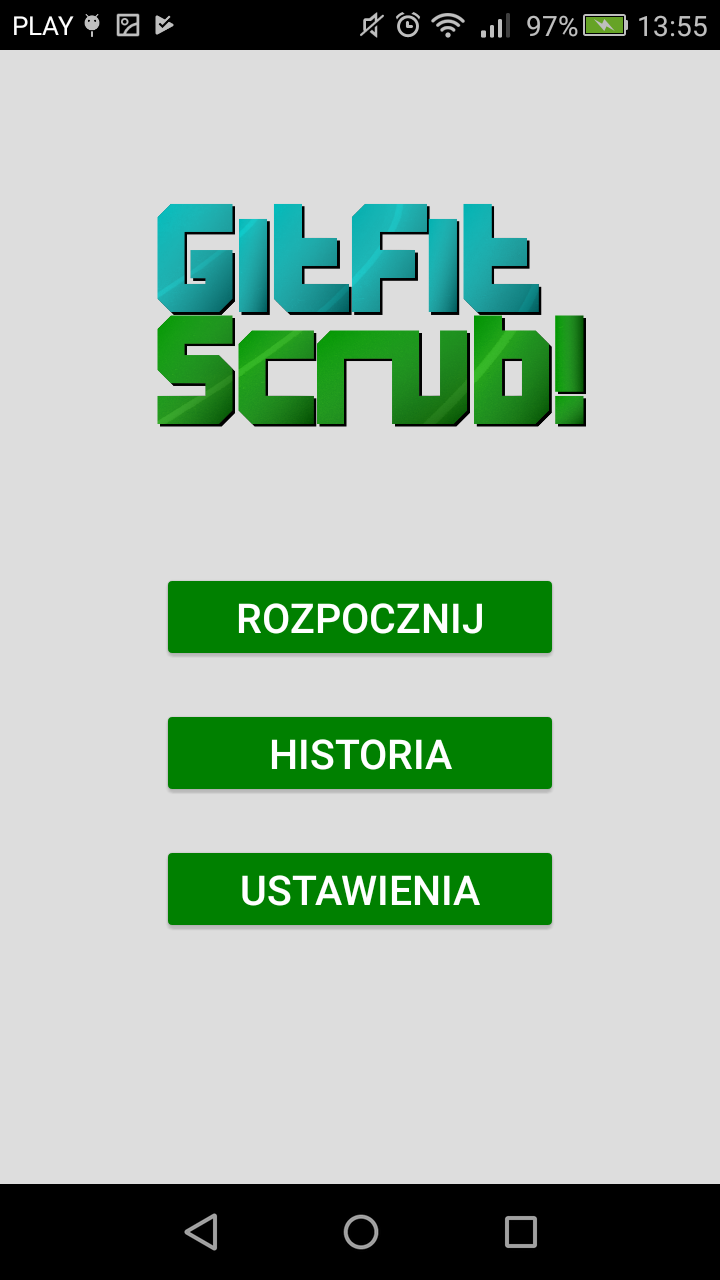
\includegraphics[height=0.6\textwidth]{img/mainMenu.png}
	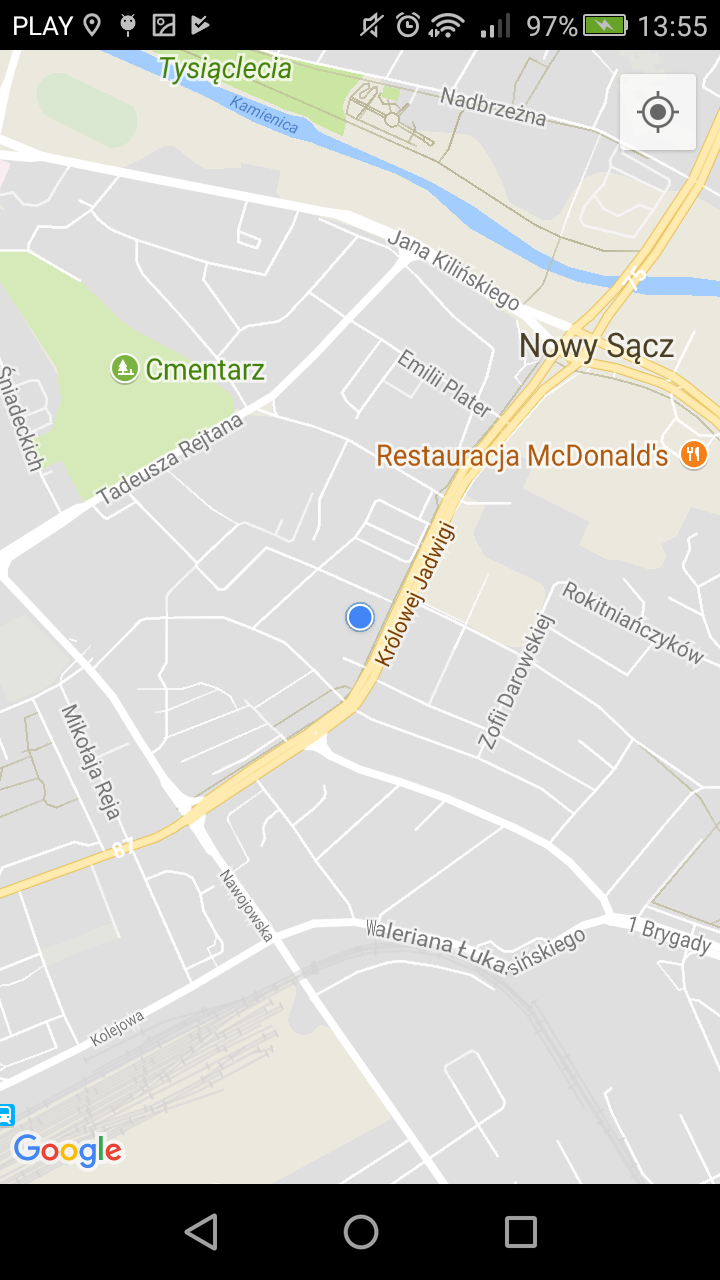
\includegraphics[height=0.6\textwidth]{img/mapsActivity.png}\\
	{Ekran menu głównego (po lewej) oraz widok mapy, po wciśnięciu przycisku "Rozpocznij", z oznaczoną pozycją urządzenia.}
    \end{figure}

\section{Sprint 2}

\subsection{Cel} Pobranie i przetworzenie danych na postawie geolokalizacji użytkownika oraz wyświetlanie wybranych informacji (średnia prędkość, czas i dystans).

\subsection{Sprint Planning/Backlog}

\paragraph{Tytuł zadania.} Stworzenie alertu o braku aktywacji modułu GPS.
\begin{itemize}
\item Estymata: M.
\end{itemize}

\paragraph{Tytuł zadania.} Pobranie informacji z modułu GPS.
\begin{itemize}
\item Estymata: L.
\end{itemize}

\paragraph{Tytuł zadania.} Stworzenie przycisku "Rozpocznij nowy trening" oraz nadanie mu funkcjonalności.
\begin{itemize}
\item Estymata: L.
\end{itemize}

\paragraph{Tytuł zadania.} Przetworzenie zgromadzonych informacji.
\begin{itemize}
\item Estymata: XL.
\end{itemize}

\subsection{Realizacja}

\paragraph{Tytuł zadania.} <<Tytuł>>.
\subparagraph{Wykonawca.} <<Wykonawca>>.
\subparagraph{Realizacja.}

\subsection{Sprint Review/Demo}
<<Sprawozdanie z przeglądu Sprint'u -- czy założony cel (przyrost) został osiągnięty oraz czy wszystkie zaplanowane Backlog Item'y zostały zrealizowane? Demostracja przyrostu produktu>>.

\section{Sprint 3}

\subsection{Cel} <<Określić, w jakim celu tworzony jest przyrost produktu>>.

\subsection{Sprint Planning/Backlog}

\paragraph{Tytuł zadania.} <<Tytuł>>.
\begin{itemize}
\item Estymata: <<szacowana czasochłonność (w ,,koszulkach'')>>.
\end{itemize}

\paragraph{Tytuł zadania.} <<Tytuł>>.
\begin{itemize}
\item Estymata: <<szacowana czasochłonność (w ,,koszulkach'')>>.
\end{itemize}

\paragraph{<<Tutaj dodawać kolejne zadania>>}

\subsection{Realizacja}

\paragraph{Tytuł zadania.} <<Tytuł>>.
\subparagraph{Wykonawca.} <<Wykonawca>>.
\subparagraph{Realizacja.} <<Sprawozdanie z realizacji zadania (w tym ocena zgodności z estymatą). Kod programu (środowisko \texttt{verbatim}): \begin{verbatim}
for (i=1; i<10; i++)
...
\end{verbatim}>>.

\paragraph{Tytuł zadania.} <<Tytuł>>.
\subparagraph{Wykonawca.} <<Wykonawca>>.
\subparagraph{Realizacja.} <<Sprawozdanie z realizacji zadania (w tym ocena zgodności z estymatą). Kod programu (środowisko \texttt{verbatim}): \begin{verbatim}
for (i=1; i<10; i++)
...
\end{verbatim}>>.

\paragraph{<<Tutaj dodawać kolejne zadania>>}


\subsection{Sprint Review/Demo}
<<Sprawozdanie z przeglądu Sprint'u -- czy założony cel (przyrost) został osiągnięty oraz czy wszystkie zaplanowane Backlog Item'y zostały zrealizowane? Demostracja przyrostu produktu>>.

\section*{<<Tutaj dodawać kolejne Sprint'y>>}


\begin{thebibliography}{9}

\bibitem{Cov} S. R. Covey, {\em 7 nawyków skutecznego działania}, Rebis, Poznań, 2007.

\bibitem{Oet} Tobias Oetiker i wsp., Nie za krótkie wprowadzenie do systemu \LaTeX  \ $2_\varepsilon$, \url{ftp://ftp.gust.org.pl/TeX/info/lshort/polish/lshort2e.pdf}

\bibitem{SchSut} K. Schwaber, J. Sutherland, {\em Scrum Guide}, \url{http://www.scrumguides.org/}, 2016.

\bibitem{apr} \url{https://agilepainrelief.com/notesfromatooluser/tag/scrum-by-example}

\bibitem{us} \url{https://www.tutorialspoint.com/scrum/scrum_user_stories.htm}

\end{thebibliography}

\end{document}

% ----------------------------------------------------------------
